\textbf{Problem 2}\\
(c). (2 points) \textsl{Observe the plot you made in Part (a) Question 1. The number of nodes increases sharply over the first few phases then levels out. Comment on what you think may be causing this effect. Based on your answer, should you adjust your conclusions in Part (b) Question 5? ($\sim$100 words, 200 word limit.)}\\

\textbf{Solution}:\\
The number of nodes and edges of the network is increasing quite fast in the first three phases (see figure \ref{fig:nodes_edges}). The seizure of 300 kg of marijuana (phase 4) might have the effect of decreasing edge numbers and stagnating node counts. The phases of seizures seem to bound the number of edges to around 50 and reduces the growth rate of node counts.\\

\begin{figure}[h]
	\centering
	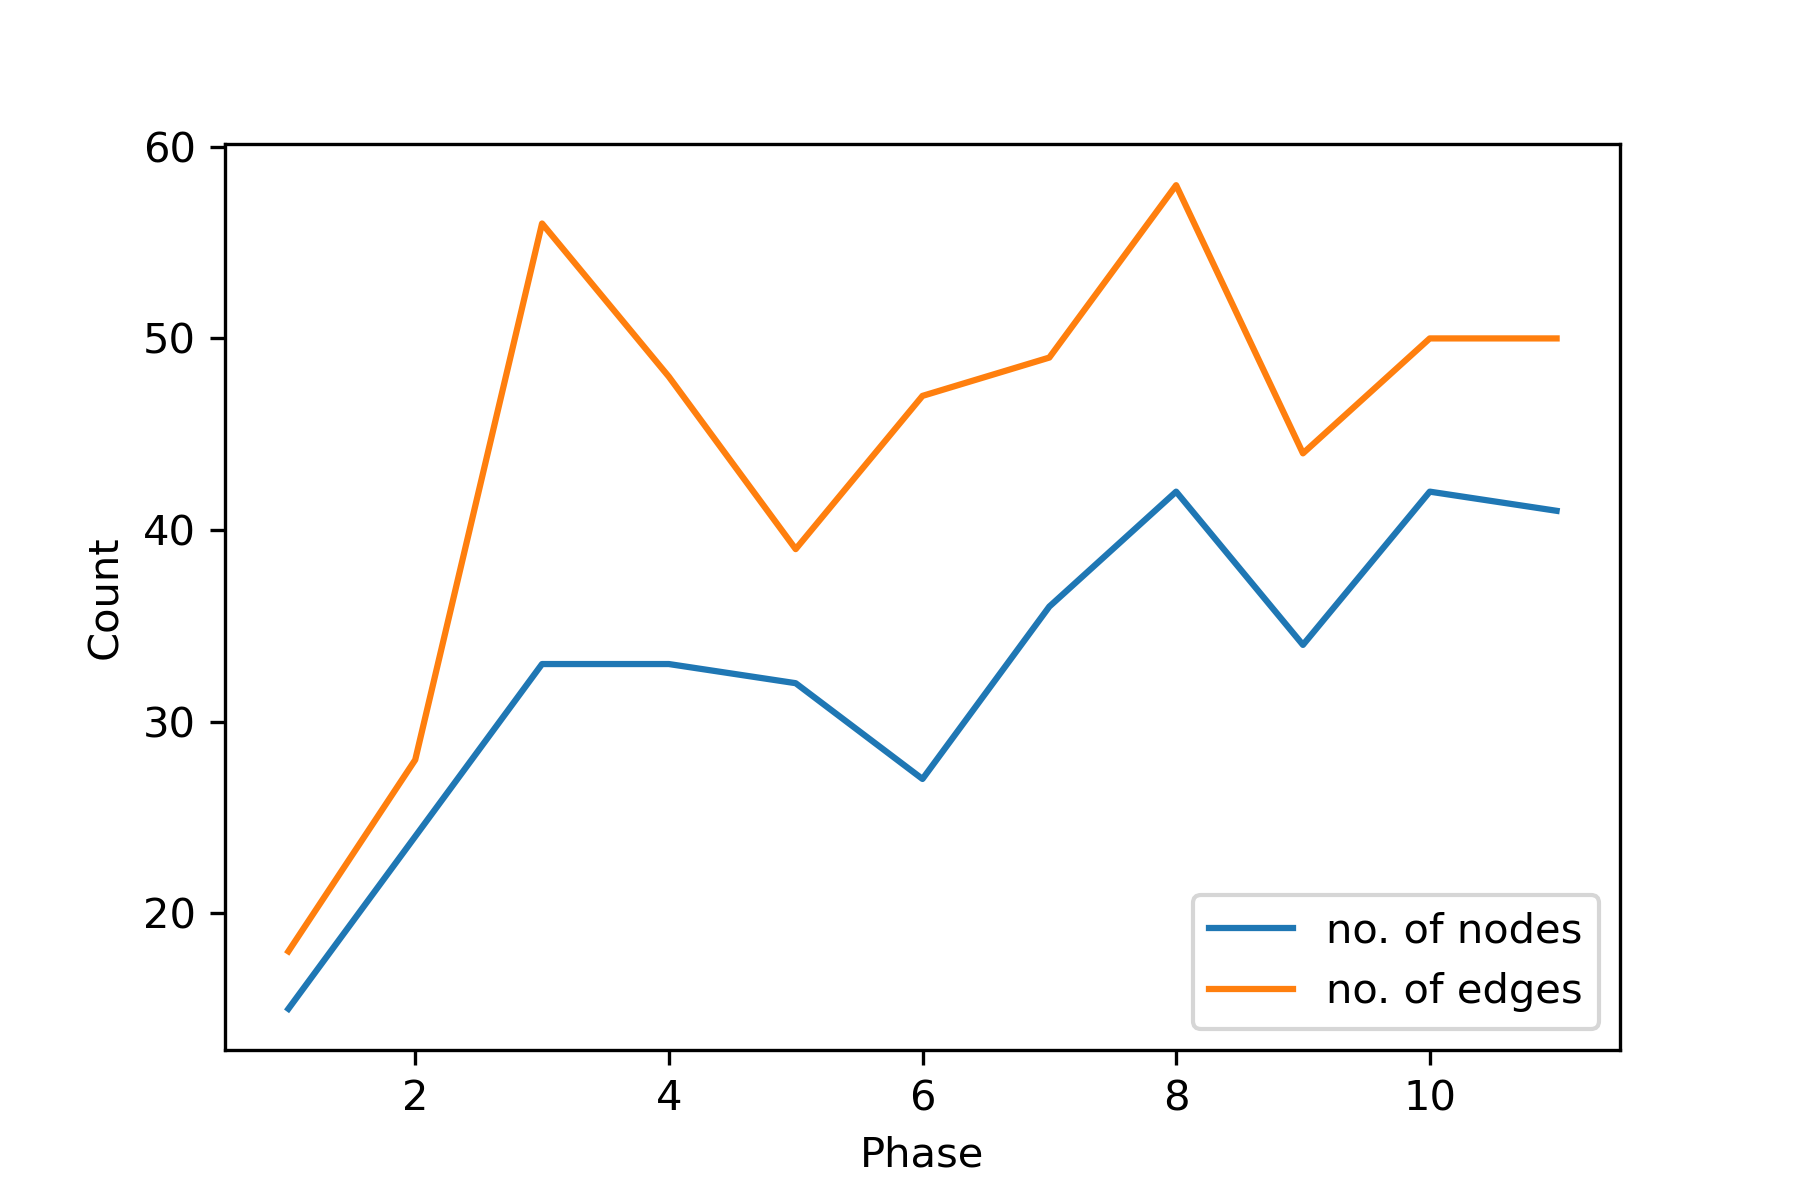
\includegraphics[width=0.7\linewidth]{problem_02/nodes_edges}
	\caption{Number of nodes and edges over phases}
	\label{fig:nodes_edges}
\end{figure}

The mean value of a centrality measure over all phases does not take into account how the individual node acts over phases. The importance of individual nodes could for example fade out over time, which is not represented by this model.\\